

\tikzset{every picture/.style={line width=0.75pt}} %set default line width to 0.75pt        

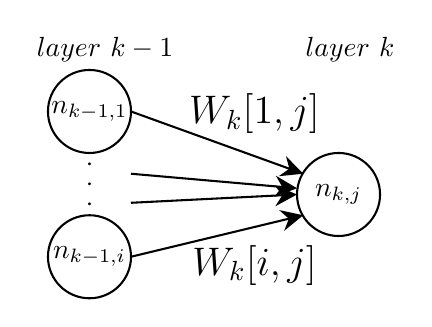
\begin{tikzpicture}[x=0.75pt,y=0.75pt,yscale=-1,xscale=1]
%uncomment if require: \path (0,300); %set diagram left start at 0, and has height of 300

%Shape: Circle [id:dp13857136549466964] 
\draw   (100,90) .. controls (100,78.95) and (108.95,70) .. (120,70) .. controls (131.05,70) and (140,78.95) .. (140,90) .. controls (140,101.05) and (131.05,110) .. (120,110) .. controls (108.95,110) and (100,101.05) .. (100,90) -- cycle ;
%Shape: Circle [id:dp8027912343340515] 
\draw   (220,130) .. controls (220,118.95) and (228.95,110) .. (240,110) .. controls (251.05,110) and (260,118.95) .. (260,130) .. controls (260,141.05) and (251.05,150) .. (240,150) .. controls (228.95,150) and (220,141.05) .. (220,130) -- cycle ;
%Shape: Circle [id:dp6531860577539721] 
\draw   (100,160) .. controls (100,148.95) and (108.95,140) .. (120,140) .. controls (131.05,140) and (140,148.95) .. (140,160) .. controls (140,171.05) and (131.05,180) .. (120,180) .. controls (108.95,180) and (100,171.05) .. (100,160) -- cycle ;
%Straight Lines [id:da3593349023905198] 
\draw    (140,90) -- (220.18,118.98) ;
\draw [shift={(223,120)}, rotate = 199.87] [fill={rgb, 255:red, 0; green, 0; blue, 0 }  ][line width=0.08]  [draw opacity=0] (10.72,-5.15) -- (0,0) -- (10.72,5.15) -- (7.12,0) -- cycle    ;

%Straight Lines [id:da8904753170585369] 
\draw    (140,160) -- (220.08,140.7) ;
\draw [shift={(223,140)}, rotate = 526.45] [fill={rgb, 255:red, 0; green, 0; blue, 0 }  ][line width=0.08]  [draw opacity=0] (10.72,-5.15) -- (0,0) -- (10.72,5.15) -- (7.12,0) -- cycle    ;

%Straight Lines [id:da007203855246534552] 
\draw    (140,120) -- (217.01,126.74) ;
\draw [shift={(220,127)}, rotate = 185] [fill={rgb, 255:red, 0; green, 0; blue, 0 }  ][line width=0.08]  [draw opacity=0] (10.72,-5.15) -- (0,0) -- (10.72,5.15) -- (7.12,0) -- cycle    ;

%Straight Lines [id:da72260506902163] 
\draw    (140,134) -- (217,130.15) ;
\draw [shift={(220,130)}, rotate = 537.14] [fill={rgb, 255:red, 0; green, 0; blue, 0 }  ][line width=0.08]  [draw opacity=0] (10.72,-5.15) -- (0,0) -- (10.72,5.15) -- (7.12,0) -- cycle    ;


% Text Node
\draw (120,125) node  [rotate=-90] [align=left] {. . .};
% Text Node
\draw (120,90) node    {$n_{k-1,1}$};
% Text Node
\draw (240,130) node    {$n_{k,j}$};
% Text Node
\draw (120,160) node    {$n_{k-1,i}$};
% Text Node
\draw (199.5,91) node  [font=\Large]  {$W_{k}[ 1,j]$};
% Text Node
\draw (199.5,164) node  [font=\Large]  {$W_{k}[ i,j]$};
% Text Node
\draw (127.5,60) node    {$layer\ k-1$};
% Text Node
\draw (245.5,60) node    {$layer\ k$};


\end{tikzpicture}
